\documentclass[a4paper,11pt,final]{report}
% Pour une impression recto verso, utilisez plutôt ce documentclass :
%\documentclass[a4paper,twoside,11pt,final]{article}

\usepackage[francais]{babel}
\usepackage[utf8]{inputenc}
\usepackage[T1]{fontenc}
\usepackage[pdftex]{graphicx}
\usepackage{setspace}
\usepackage[colorlinks=true,linkcolor=black,urlcolor=blue]{hyperref}
\usepackage[french]{varioref}
\usepackage[top=7em, bottom=7em, left=7em, right=7em]{geometry}
\usepackage{wrapfig}
\usepackage{fancyhdr}
\usepackage[nottoc, notlof, notlot]{tocbibind} % biblio dans table des matières
\fancyhf{}
\renewcommand{\footrulewidth}{0.05em}
%entete
\lhead{\leftmark}
%pied depage
\cfoot{\thepage}
\lfoot{}
\rfoot{Desserte Robotisée}

\newcommand{\reporttitle}{Desserte Robotisée}     % Titre
\newcommand{\reportauthor}{Louis \textsc{LE CLEC'H}\\
                           Théophile \textsc{GUILBAUD}\\
                           Clément \textsc{BRISSET}}% Auteur
\newcommand{\reportsubject}{Environnement, démarche, et conception} % Sujet
\newcommand{\HRule}{\rule{\linewidth}{0.5mm}}
\newcommand{\siecle}[1]{\textsc{\romannumeral #1}ème}
\setlength{\parskip}{1ex} % Espace entre les paragraphes


\hypersetup{
    pdftitle={\reporttitle},%
    pdfauthor={\reportauthor},%
    pdfsubject={\reportsubject},%
   % pdfkeywords={rapport} {vos} {mots} {clés}
}

\begin{document}
  \begin{titlepage}
\begin{flushleft} 
  \large
  \emph{Auteur :}\\
  \reportauthor\\
\end{flushleft}
\begin{center}
  
  \begin{center}
    \begin{tabular}{c}
      \\
      
\includegraphics [width=60mm]{Images/ENSEIRB-MATMECA.jpg} \\
      \\
      
\includegraphics [width=70mm]{Images/logo-INRIA.jpg}\\
      \\
      \\
    \end{tabular}
    
    
      
    \textsc{\Large \reportsubject}\\[0.5cm]
           {\large 9 janvier au 28 janvier}\\
           
           
           \HRule \\[0.4cm]
                  {\huge \bfseries \reporttitle}\\[0.4cm]
                  \HRule \\[1.5cm]
                  
                  \begin{center}
                    
                    
                    
                    
                  
                  
                  %\vfill                  
                  
                  
                  
  \end{center}    
\end{center}
\begin{flushbottom}
\begin{flushright} 
  \large
  \emph{Responsables :} \\
  M.~David DANEY - \small{INRIA} \\
  M.~Christian MALAURIE - \small{Bordeaux 3}
\end{flushright}
\end{flushbottom}
\end{center}
\end{titlepage}

  %\cleardoublepage % Dans le cas du recto verso, ajoute une page blanche si besoin
  \tableofcontents % Table des matières
  \listoffigures
 % \sloppy          % Justification moins stricte : des mots ne dépasseront pas des paragraphes
  %\cleardoublepage
  \begin{onehalfspace}
  \pagestyle{fancy}

\chapter*{Introduction}
\addcontentsline{toc}{chapter}{Introduction}

%surement qu'il faudrait mettre le classique de la réalisation de tte introduction: accroche , problématique, analyse du devellopement du plan

\section{Comment concevoir dans un champ social}
%Ouaouh! on a construit des robots pour aller sur la lune mais le mettre avec des humains c'est plus difficile

L’industrie, la technique et la recherche sont déjà investies par les robots. Mais quand les considérerons-nous comme des partenaires à part entière de notre vie ? C’est à cette question que tend à répondre ce projet de desserte robotisée.

C’est à l’origine dans le domaine de l’industrie, notamment automobile, que les robots se sont d’abord et le plus durablement installés. Pour ensuite se trouver dans les zones nucléaires, les terrains minés, l’espace ou les abysses marins à très forte pression. Et c’est ainsi que le robot a su se faire une place dans ces milieux dit « extrêmes ». Mais il n’est pas encore très bien adapté au secteur du service.

Faire entrer un robot chez soi reste pour beaucoup un grand pas à franchir. Il faut donc réussir à faire rentrer le robot dans notre société de façon subtile. Alors l’acceptation du robot comme un atout pour l’être humain, et non comme un danger, deviendra possible.

A travers la desserte robotisée, nous offrons au robot une place de soutiens au service lors de cocktail. On l’intègre donc à une place de partenaire pour l’homme. Et c’est ainsi qu’il prend une place dans le champ humain sans s’y imposer de façon brusque.


\section{Le context du cocktail}

\subsection{Où se déroule un cocktail}
%lister les lieux

\subsection{Qui sont les acteurs du cocktail}
%lister les personnes

\subsection{Les ambiances d'un cocktail}
%lister les qualités

\subsection{Les complexités des niveaux d'intéractions dans le cocktail}
%lister les "`enjeux"' qui amènent les intéractions


 
\chapter{Objectif}

La création de la desserte robotisée a pour but de créer un compromis au serveur de cocktail. Notre but est de le rendre non pas le plus humain possible mais le plus serviable et utile. C’est pourquoi il n’est pas un serveur à part entière mais un objet mobile avec une intelligence lui permettant de s’occuper des besoins des convives, un robot. Il ne doit donc pas s’imposer à l’atmosphère du cocktail mais bien en faire partie.

\section{Servir les invités}
%"'comprendre"' le client

Le robot a pour objectif principal de permettre le service d’apéritifs aux convives. Il doit donc se déplacer entre les invités et leur apporter les amuse-bouches et le champagne.C’est pourquoi, avant même le service, il est capable de savoir ce qu’il doit avoir sur son plateau. Il ne peut pas savoir ce que ses clients veulent mais il sait ce que le cocktail a promis à ses hôtes. C’est pourquoi il a un planning de son service dans le but de satisfaire les invités.
//
Lors d’un cocktail, les gens se réunissent autour de groupe de personne qu’il connaissait ou qu’il rencontre, il y a donc des formations de groupes. Le robot doit les repérer et réaliser son service. Pour réussir cet objectif, il devra suivre des conventions de service. Comme le serveur qui apporte les mets sans s’introduire dans le cocktail, le robot doit être capable de présenter les apéritifs et savoir lorsque les personnes dont ils s’occupent sont servies. 
//
Lorsque le service et réalisé, si un hôte peut lui demander de venir le servir. Si ce n’est pas le cas, il retourne à sa déambulation.
//
Pour assurer avec brillance son service, il doit permettre d’être un atout à la réussite du contexte social du cocktail. C’est-à-dire qu’il doit être un gain de temps pour ses convives pour qu’ils puissent réaliser leurs objectifs tel que les rencontres où les retrouvailles. C’est pour cela qu’il a assez d’éléments sur son plateau pour satisfaire le plus de personne ; qu’il se déplace de tel sorte que le plus de personnes soient servis et, qu’à travers le robot, les clients trouvent toutes les informations nécessaires sur le cocktail. Ainsi le robot aura réussi à valoriser toutes les personnes se trouvant dans le cocktail.

%désirs de performance -> Avoir tout sur le plateau, Gagner du temps, avoir des infos

\section{être un lien de communication}

En plus d’être un élément de service, le robot est intrinsèquement un élément de communication. Sans agir sur les relations qu’auront les personnes entre elles, il doit pouvoir s’adapter aux mouvements de formation de groupes et avoir la possibilité d’en être le créateur.
//
Lors du début d’un cocktail, les groupes ne sont pas formés. Au cours de l’évènement, les gens se rassemblent et au fur à mesures que le cocktail se déroule seuls quelques électrons libres continue de passer de groupes en groupes. On a donc en début de cocktail des gens très dispersés. Et à la fin du cocktail on retrouve un ensemble de groupe.
//
Pour rendre le robot utile lors de se développement du cocktail, il faut que le robot   est la capacité de réunir les gens. Il est un élément d’échange entre les convives.


%adaptation du design

%Etre un éléments d'échange entre les convives
%Mettre en relation les convives
%Permettre à deux convives d'échanger discrètement
%Se faire accepter par l'humain 

\chapter{Contraintes et Propriété}

\section{Les contraintes anthroposociales}

Les contraintes anthroposociales imposées à la conception d'une desserte robotisée destinée aux cocktails peuvent être séparées en plusieurs catégories :
\begin{description}
\item[sensorielles :]
  \begin{enumerate}
  \item Le robot ne doit pas par sa présences déranger le bon déroulement des conversations entre convives.
  \item L'apparence du robot doit être en accord avec l'ambiance et le code vestimentaire du cocktail.
  \item La promité du robot ne doit pas induire de sensations désagréables
  \end{enumerate}
\item[confiances :]
  \begin{enumerate}
  \item Le robot doit respecter les distances nécéssaires afin de ne pas pénétrer l'espace personnel des convives.
  \item Le robot doit être prévisible afin de ne pas effrayer les convives et de renforcer le sentiment de sécurité à sa périphérie.
  \item Le gabarit du robot doit être soigneusement réfléchie afin de ne pas paraitre comme le dominant de l'interaction aussi bien que pour empêcher une apparence menacante.
  \end{enumerate}
\end{description}

%espace perso
%gène du robot (cmt se faire accepter par l'humain) #AvoirUneEmpriseCorporelSurLeRobot
%Confiance (et non pas sécurité)
%Plaisant

%Petite aide:
%ds le context du cocktail on est vigilant => on est "`fin"' dans nos actions


\section{Les contraintes techniques}

\subsection{Contraintes déduitent du champ social}


\begin{description}
\item[sensorielles :]
  \begin{enumerate}
  \item Le niveau sonore émit par le robot ne doit pas excéder les XX (niveau sonore à déterminer) décibel.
  \item La forme du robot devra être affinée le plus possible et disposer de carénages amovibles permettant de s'adapter à différentes ambiances ainsi que la création de carénages customisé par le client, si celui-ci le souhaite.
  \item Afin de ne pas incommoder les convives et leur expérience, le robot ne devra pas dégager trop de chaleur ni d'odeur.
  \end{enumerate}
\item[confiances :]
  \begin{enumerate}
  \item Le robot devra embarquer des capteurs et le software nécéssaire au maintient des distances programmées avec les convives.
  \item Les mouvements devront être fluide, et un ensembles de mouvement plus ou moins évident devront être déterminé et implémenter afin de laisser savoir au personnes alentour les intentions du robot.
  \item Le robot ne devra pas excéder une tailler de 1m50 et une circonférence de 3m, ceci afin de rester dans une position de servant par rapport aux convives.
  \end{enumerate}
\end{description}

%bruit
%chaleur
%grandeur

\subsection{Faisabilité}

%sécurité
%durabilité
%batterie

\section{Les propriétés}
%not sure
\subsection{Caractéristique}
%not sure


\chapter{Spécification fonctionnelle}

\section{Les tâches principales}

\subsection{Se déplacer}

Le déplacement est bien entendu un élément cruciale de la conception
d'un robot. La desserte robotisée a ceci de particulier qu'elle doit
évoluer en milieu humain. Cela demande de définir exactement quand le
robot est en risque de rencontrer des humains, et comment il doit
réagir.

Au dela de cet aspect, nous devons également définir tous les types de
déplacements que le robot devra effectuer:

\begin{itemize}
\item Construction de carte
\item arrivée en salle
\item déambulation
\item gestion de groupe
\item suivi
\item dirigé
\item retour à la base
\item utilisation de l'interface
\end{itemize}

\subsubsection{Mode construction de carte}
La construction de carte est l'action primaire du robot lui permettant par la suite de se repérer dans la salle. C'est pourquoi elle doit se dérouler avant l'arrivée des convives ou après leur départ. C'est durant cette phase que le robot crée un carte de la salle de cocktail dans laquelle il va devoir se déplacer. Ainsi, lors de la réception, il pourra savoir se positionner dans la salle de réception.

La phase de construction de carte se déclenche par un élément externe comme le maître de réception. Pour déclencher se mode il faut que le robot soit dans la salle à cartographier. C'est à dire que le robot peut y être présent avant le lancement d'un autre mode de déplacement ou après avoir suivi la personne qui enclenchera le mode, soit après le mode suivi.

la cartographie se réalise à l'aide de deux caméra. Le robot se déplace seulement pour peaufiner sa carte. Sinon le robot tourne sur lui-même pour réaliser sa carte de repère. Ce mode se termine lorsque le robot a réalisé sa carte. 

Après avoir enclenché réalisé la carte, le robot devra rentrer à sa base avant le lancement de la soirée cocktail.

Les points d'entrées du mode sont:
\begin{itemize}
\item aucun mode
\item Le mode suivi
\end{itemize}

Les points de sorties du mode sont:
\begin{itemize}
\item le mode retour à la base.
\end{itemize}

\subsubsection{Mode arrivée en salle}

Le déplacement de la base vers la salle est la première chose que doit réaliser 
le robot avant de commencer sa déambulation. C’est donc  le moment où il vérifie 
que ses batteries sont chargées, que son plateau est rempli et qu’il connait le 
chemin vers la salle. Le mouvement de la base vers la salle peut être déjà cartographié.
Cet évènement ne peut arriver que s’il est déjà à sa base.

Les points d'entrées du mode sont:
\begin{itemize}
\item Le mode retour à la base
\item Le mode dirigé
\item Le mode suivi
\end{itemize}

Les points de sorties du mode sont:
\begin{itemize}
\item le mode déhambulation.
\end{itemize}


\subsubsection{Mode déambulation}

Le mode déambulation est l'un des princpaux mode de déplacement de la
desserte. Il s'agit pour le robot de repérer un groupe de convive puis
de se déplacer vers lui. Un des point clé de ce déplacement est que le
robot doit éviter de retourner sur une zone géographique qu'il à déjà
servi.

le déroulement du mode se fait comme suit:
\begin{itemize}
\item déclenchement du mode à l'arrivée dans la salle.
\item la disserte va de groupe en groupe et le cas échéant de table en
  table.
\item le robot garde en mémoire les zones géographiques déjà
  desservies et priorise les zones encore non servie.
\item Fin du mode de déambulation à la fin d'un timer et/ou après une
  diminution significative du poids du plateau, ou en cas d'absence
  d'espace ou passer (interieur d'un groupe), ou en cas de rencontre
  d'un groupe.\\
\end{itemize}

les points d'entrée du mode sont:
\begin{itemize}
\item le mode utilsation de l'interface
\item le mode arrivée en salle
\item le mode suivi
\item le mode dirigé\\
\end{itemize}

les points de sorties du mode sont:
\begin{itemize}
\item le mode suivi
\item le mode dirigé
\item le mode retour à la base
\item le mode gestion de groupe
\item le mode utilisation de l'interface\\
\end{itemize}

\subsubsection{Mode gestion de groupe}
Le mode de gestion de groupe est destiné au service d'un groupe de personnes. Suite à la prise de décision du robot de servir un groupe qu'il a détecté. Celui-ci rentre dans ce mode avant d'effectuer le service. Celui-ci commence par déterminer une hiérarchie dans le groupe lui permettant d'établir l'ordre le plus efficace et socialement correct pour servir les convives. La sortie du mode s'effectue une fois le service terminée.\\

Les points d'entrées du mode sont :
\begin{itemize}
\item mode déambulation
\end{itemize}

Les points de sortie du mode sont :
\begin{itemize}
\item mode déambulation
\end{itemize}

\subsubsection{Mode suivi}
Le mode suivi est un mode qui peut uniquement être activé et désactivé de façon manuelle via le mode utilisation interface.
Celui-ci est destiné à une utilisation exceptionnelle pour des cas spéciaux.

On pourra imaginer un mécanisme de sécurité implémenté dans l'interface qui permettra uniquement à des personnes habilitée d'activer ce mode de déplacement.
Une fois le mode activer, un émetteur amovible sera libéré et mis à la disposition de la personne ayant activer le mode.
Après activation du mode, le robot suivra cette émetteur en gardant une certain distance de sécurité, afin qu'en évitant tout se qui pourrait venir se placer dans son chemin. Cela permet donc d'emmenner le robot à n'importe quel endroit souhaité, par exemple une zone de chargement spéciale éloigné de la base du robot.\\


Les points d'entrées du mode sont :
\begin{itemize}
\item mode utilisation interface
\end{itemize}

Les points de sortie du mode sont :
\begin{itemize}
\item mode utilisation interface
\end{itemize}

\subsubsection{Mode dirigé}
Le mode dirigé permet au robot de faire des dessertes spéciales transmise par l'ordinateur centrale.
Cet ordre peut avoir été passé par le maitre d'hotel tout comme par un convive, demandant à un certain robot de changer de section, ou bien d'aller deservir une table ou un groupe particulier.
On peut aussi envisager de lui faire livrer une commande spéciale.\\

Le déroulement du mode se fait comme suit:
\begin{enumerate}
\item Commande reçue par l'ordinateur centrale
\item L'ordinateur centrale determine le meilleur robot pour effectuer la desserte
\item Si besoin, le robot choisie va à sa base pour récupérer ce dont il à besoin
\item Le robot effectue la desserte demandé\\
\end{enumerate}


Les points d'entrées du mode sont :
\begin{itemize}
\item mode déambulation
\item mode arrivée en salle
\item mode retour à la base
\end{itemize}

Les points de sortie du mode sont :
\begin{itemize}
\item mode déambulation
\item mode arrivée en salle
\item mode retour à la base
\end{itemize}

\subsubsection{Mode retour a la base}

Ce mode permet au robot de rentrer à la base lorsqu'il en a besoin
(ravitaillement, disfonctionnement, rappel du maitre d'hotel...).

le déroulement du mode se fait comme suit:
\begin{itemize}
\item déclenchement lorsque le plateau est vide et/ou timer, en cas de
  detection d'anomalie, ou de rappel à la base.
\item en cas de déplacement impossible, envoie une demande demande
  d'assistance.
\item cherche le plus court chemin ne passant pas par des groupes
\item fin du mode lorsque le robot arrive à la base.\\
\end{itemize}

les points d'entrée du mode sont:
\begin{itemize}
\item le mode déambulation
\item le mode utilsation de l'interface
\item le mode arrivée en salle
\item le mode suivi
\item le mode dirigé\\
\end{itemize}

les points de sorties du mode sont:
\begin{itemize}
\item le mode suivi
\item le mode dirigé
\item le mode utilisation de l'interface\\
\end{itemize}

\subsubsection{Mode utilisation interface}
Le robot entre dans ce mode lorsque quelqu'un utilise une des
interfaces du robot. Dans ce cas le robot doit cesser de se deplacer.

\subsection{schéma générale}

\begin{figure}[h]
\begin{center}
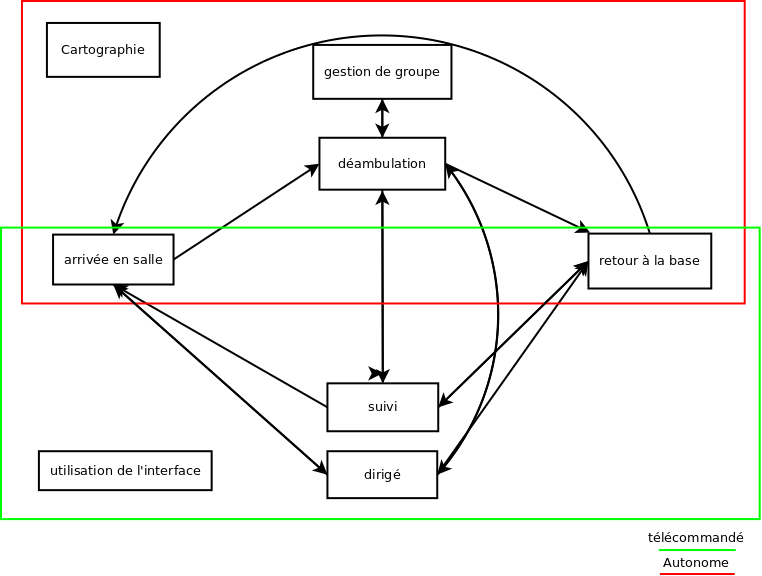
\includegraphics[scale=0.55]{Images/transition_mode.png}
\caption{Transition des modes}
\label{Transition des modes}
\end{center}
\end{figure}

\subsection{Servir}

\subsubsection{Maintenir le plateau}

\subsubsection{Presenter le plateau}

\subsection{Communication}
 


\section{Les tâches secondaires}

Les tâches principales du robot étant réalisé, il est toujours possible d’améliorer le robot en lui rajoutant des fonctionnalités pour réaliser des taches secondaires. C’est tâches ne seront pas détaillé par soucis de temps pour la réalisation de ce projet mais il serait intéressant d’y repenser. Pour vous aider dans vos réflexions, nous avons noté quelques idées.

\subsection{\^Etre un éléments d'échange entre les convives}

Le robot devrait pouvoir être un élément d’échange entre les convives. Il pourrait par exemple avoir des jeux sur lui ou des situations de rassemblement.

\subsubsection{Permettre à deux convives d'échanger discrètement}

Le robot pourrait être le messager discret entre deux convives.


\chapter{Spécification techniques}

\section{Le Hardware}

\subsection{Le bras}

Pour assurer les mouvements de service et pour ranger le plateau lors
des déplacement un bras robotisé avec trois degrés de liberté est
suffisant pour reprendre les gestes d'un serveur, il devra cepandant
avoir comme caractéristique la possibilité de se retracter pour ranger
le plateau en position de déplacement.

Le plateau disposera également de capteur à ultrasons et/ou infrarouge
pour permettre de positionner le plateau aux bonnes distances par
rapport aux groupes ou aux personnes, soit un peu moins d'un mètre.
Cela implique cependant que le robot arrive à faire la différence entre 
une personne désirant se servir et une personne n'ayant pas vu le robot 
et ayant une trajectoire dangeureuse.

le plateau comme annoncé dans les contraintes liées au services a
traditionnellement un diamètre de $40cm$ que nous avons décidé de
conserver. Comme il doit être composé d'une matière disposant d'un
bonne isolation thermique, une base en acier inoxydable nous semble
être une solution cohérente.

Un capteur de pression devra être installé sur le plateau pour déterminer 
a quel moment le plateau doit être recharger.

\subsection{Le corps}

\subsubsection{Chassis}
Nous avons choisis de donner au robot un corps cylindrique d'un
diamètre légerement supérieur $45cm$. l'idée étant qu'en position de
déplacement, le plateau s'emboite légèrement dans le corps du robot.
La matière composant l'exterieur du chassis devras être relativement
souple pour minimiser un impact qui n'aurait pas pu être éviter. 

\subsubsection{Base mobile}
Pour ce qui est de la base mobile, nous avons choisi l'utilisation de
roue omnidirectionnelle, car les déplacements du robot demandent une
grande précision du fait de l'évolution en milieu humain, par contre
ce choix impose un sol totalement plat, ce qui exclut d'office tout
service en milieu exterieur.

\subsubsection{Sécurité}
Pour répondre aux contraintes de sécurités, nous nous somme inspirés
du robot numéro 1 (voir le chapitre sur l'état de l'art) et nous avons
choisis de coupler des capteur infrarouges à des capteurs à ultrasons
disposé tout autour du chassis pour permettre au robot d'éviter tout
contact. 

\subsubsection{Interface}
une surface tactile est prévue pour permettre à un utilisateur
d'interagir avec le robot (par exemple pour obtenir des information).

\subsubsection{autonomie}

\subsubsection{Caméra}

Outre les différents capteurs déjà cité pour le plateau ou la sécurité
du robot, une ou plusieurs caméras doit être installée sur le robot pour l'aider
d'une part à repérer des groupes de personnes, et d'autre part une
fois que le robot commence à servir le groupe, à éviter que le robot
aille servir trop de fois la même personne.

\subsubsection{}


\section{Le Software}


\section{design}


\chapter*{Annexe}
\addcontentsline{toc}{chapter}{Annexe}
\chapter{état de l'art}
Nous avons recherché plusieurs projet proche de la desserte robotisée.

\section{Robot Numéro 1 de Firstclass Robotics}
Ce projet est très proche de notre desserte d'un point de vue fonctionnel. En effet, il est prévu pour servir lors de reception. il est déjà en service et peut être loué au près de First Class Robotique. 

\begin{figure}[h]
\begin{center}
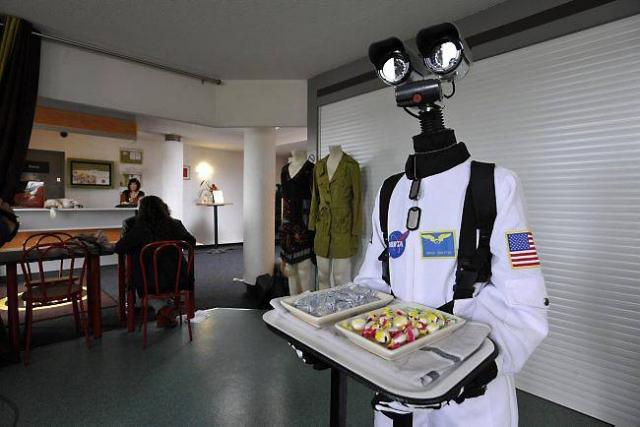
\includegraphics[scale=0.55]{Images/robot_n1.jpg}
\caption{robot Numéro 1}
\label{robot Numéro 1}
\end{center}
\end{figure} 

Ce robot à été conçu par Bernard MARTI, qui à notamment été professeur
de robotique à l'INSA de Lyon. Ce robot à clairement été conçu d'un
point de vue industriel et dans une optique de faire un robot à bas
coût. Il coute 15000 euros.

\subsection{caractéristique}
le robot fait 1m55, à une autonomie de 12h, et utilise un système de
vision basé à la fois sur des capteur infrarouge et et des capteurs
ultrasons et permettant une vision à 12m.

Le robot ce caractèrise aussi par une absence de communication avec
une base, permettant de le rendre insensible à tout pratage
informatique. il est complètement autonome et ne necessite pas de
cartographie. Bernard MARTI parle d'ailleur de programmation
insectoïde et réduite au minimum.

A noté qu'une version "plus" existe également, plus axée assistance.

\subsection{contexte}

Une différence majeure de ce robot par rapport à notre projet est que ce robot n'essaye pas d'imiter un serveur, mais se presente plutôt comme un robot d'aide au serveur. Le concepteur du robot indique par ailleurs que le robot à été plutôt bien accueilli par les professionel qui officiait a ses côtés. 

\section{Care O Bot}

Le care O bot s'écarte un peu de notre projet mais reste à étudier. Il
s'agit d'un robot d'aide à la personne, équipé d'un bras articulé et
d'un plateau. il est construit par Fraunhofer, une entreprise
allemande.

\subsection{caractéristique}

\begin{figure}[h]
\begin{center}
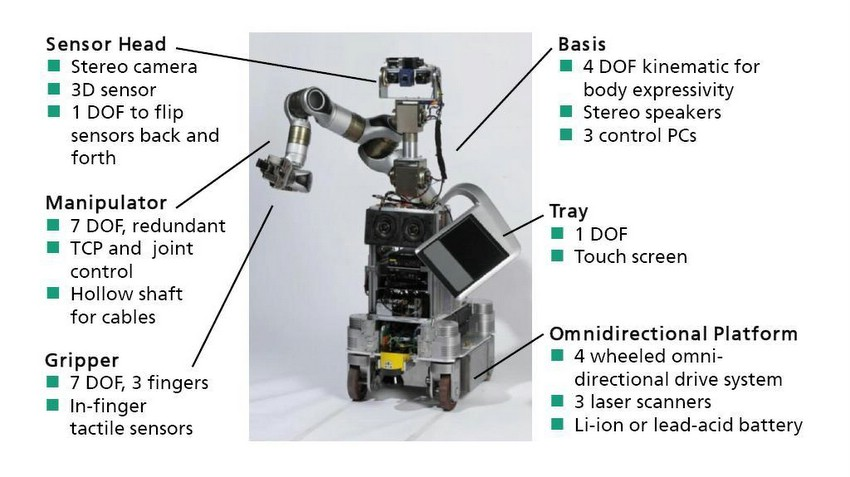
\includegraphics[scale=0.55]{Images/cob3-hardware.jpg}
\caption{caractéristique du careObot3}
\label{caractéristique du careObot3}
\end{center}
\end{figure}

Le robot roule d'une manière lente et fluide. Il utilise des caméras et des capteur de profondeurs pour se reperer, ainsi qu'un système de cartographie. Son bras possède 7 degré de liberté. pour intéragir, il dispose d'une tablette tactile sur son plateau ainsi que d'une reconnaissance faciale et auditive. Il dispose aussi d'haut parleur pour communiquer.

\subsection{contexte}

Ce robot évolue dans un contexte très différents de notre desserte. Il se trouve chez des particuliers ou dans des maisons de retraites. Il n'a donc pas les mêmes contraintes en terme de gestion de foule et de déplacement. En revanche il peut-être très interessant d'étudier sa façon de servir et de s'approcher des humains.

\section{Dalu Robot}

Dalu Robot n'est pas un robot, mais un restaurant chinois qui utilise plusieurs robot pour servir leurs clients. Ces robot sont assez rudimentaires en soi, puisqu'ils suivent une ligne blanche au sol qui fait le tour de la pièce et s'arretes losrqu'un humain s'arrête.

\begin{figure}[h]
\begin{center}
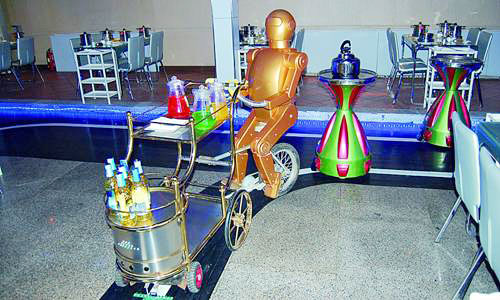
\includegraphics[scale=0.55]{Images/dalu-robot-1.jpg}
\caption{exemple de robot chez Dalu Robot}
\label{exemple de robot chez Dalu Robot}
\end{center}
\end{figure}



\chapter{\'Etude de cas}

Le vendredi 24 janvier, notre équipe a été invitée à un cocktail au sein de l’Union Régional des Ingénieurs et Scientifiques d’Aquitaine organisé par l’association Ricard. Durant ce cocktail nous avons pu faire une étude du terrain et poser des questions aux serveurs.

La soirée débuta vers 19h, il y avait 90 personnes pour une superficie avoisinant les $80m^2$, deux buffet garnit de différents alcools et 3 serveurs. Deux étaient en salle et le dernier serveur faisait la liaison entre la cuisine et la salle. Les mets étaient préparés et chauffés avant le début du cocktail.

En ce début de soirée, le niveau sonore se trouvait au environ de 65 décibels. Les pics étaient à 75 décibels et le niveau minimum à 64 décibels. Les serveurs servaient l’alcool. Les groupes se formaient entre les connaissances.

Les serveurs étaient courtois et pouvaient discuter. Il ne rentrait pas dans les groupes, c’était les groupes qui s’ouvraient à eux. Les personnes les plus enfoncés dans la salle se rapprochaient parfois pour être servi. Il ne s’approchait pas de groupe lorsque ces personnes semblaient avoir une discussion trop sérieuse.

Après le service de l’alcool, il y eut les mets froids, pendant que les buffets ne servaient que de l’alcool. Il était possible de trouver deux poubelles sur les buffets.

Ensuite vient les mets chauds. Les serveurs se déplaçaient dans la salle. Pour s’introduire plus profondément dans la salle, il levait leurs plateaux au-dessus des gens et  indiquait leurs passages par des gestes subtiles. Par exemple, il pouvait toucher discrètement le dos d’une personne avec le dos de leurs mains pour indiquer à la personne de la laisser passer. L’acte était assez bien réaliser pour que la personne ne remarque pas qu’elle se bougeait pour le serveur et pour qu’elle puisse continuer sa conversation sans être dérangé par le serveur.

Après les plats chauds, la salle se vida un peu. Nous nous retrouvions à 76 personnes. Les groupes se dissociaient pour permettre les discussions entre les gens qu’ils n’ont pas pu voir durant la soirée. Le bruit restait à la même intensité. Il y avait moins de monde mais surement que l’alcool faisait monter le ton.

C’est vers 21h que le service des pâtisseries arriva. Après ce service, la salle se vida et les serveurs commencèrent à nettoyer et les gens restant, environs 50, aidèrent à ranger la salle.

Ensuite nous avons pu discuter avec les serveurs sur le maintien du plateau, la manière dont il se déplacé dans le cocktail et comment le cocktail était préparé. 

\end{onehalfspace}


\nocite{*} 
\renewcommand{\refname}{Bibliographie}
\bibliography{biblio}{}
\bibliographystyle{ieeetr}

\end{document}
